\chapter{Process Control Engineering}
\label{Chapter:Controls}

There are two main goals in process control engineering:
\begin{enumerate*}
    \item Reference tracking, where a process variable is matched to a set-point which may be changed over time; and 
    \item Disturbance rejection, where the process variable is held to the set-point despite outside influence upsetting it;
\end{enumerate*}
This is usually achieved by a controller which measures the system inputs \andor outputs using a sensor/transmitter and controls the process variable by manipulating an actuator. 

\section{Feedback}
\begin{figure}[!ht]
    \centering
    
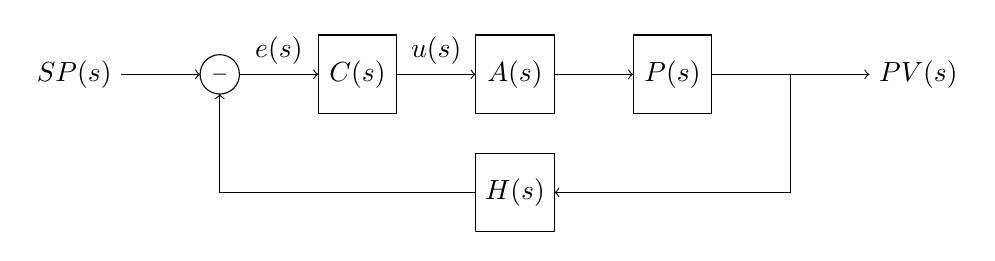
\begin{tikzpicture}
    
    %Sum
    \draw[->] (-3,0) node[anchor=east]{$SP(s)$}-- (-2,0);
    \draw (-1.75,0) circle (0.25)node{\scriptsize$-$};
    %Controller
    \draw[->] (-1.5,0) -- (-0.5,0)node[pos=0.5,anchor=south]{$e(s)$};
    \draw (-0.5,-0.5) rectangle (0.5,0.5) node[pos=0.5]{$C(s)$};
    \draw[->] (0.5,0) -- (1.5,0) node[pos=0.5,anchor=south]{$u(s)$};
    %Actuator
    \draw (1.5,-0.5) rectangle (2.5,0.5) node[pos=0.5]{$A(s)$};
    \draw[->] (2.5,0) -- (3.5,0);
    %Process
    \draw (3.5,-0.5) rectangle (4.5,0.5) node[pos=0.5]{$P(s)$};
    \draw[->] (4.5,0) -- (6.5,0) node[anchor=west]{$PV(s)$};
    %Transducer
    \draw[->] (5.5,0) -- (5.5,-1.5) -- (2.5,-1.5);
    \draw (1.5,-2) rectangle (2.5,-1) node[pos=0.5]{$H(s)$} ;
    \draw[->] (1.5,-1.5) -- (-1.75,-1.5) -- (-1.75,-0.25);
\end{tikzpicture}

    \caption[Feedback control loop]{Feedback control loop. The process-variable ($PV$) is measured by the transducer ($H$) and compared to the set-point ($SP$). The controller ($C$) uses the actuator ($A$) to control the process ($P$) based on the error ($e$).}
    \label{fig:tikz_feedback}
\end{figure}

The most common type of controller is a feedback controller. Fig. \ref{fig:tikz_feedback} shows a simple feedback control loop with an output sensor/transmitter (\ie transducer), controller, and actuator working together to control a process. The controller takes action (u) based on the `error' ($e$) between the set-point ($SP$) and process-variable ($PV$) (\ref{eqn:error}). These systems are typically modeled using transfer functions in the Laplace (or `s') domain.

\begin{equation}\label{eqn:error}
    e(t) = PV(t) - SP(t)
\end{equation}

The action, or controller output ($u$) is often determined by a \acf{pid} equation (\ref{eqn:pid}), which considers the instantaneous, cumulative, and predictive error in determining the proper actuation \cite[Ch. 5]{Bequette}. This equation has three terms:
\begin{enumerate}
\item Proportional control term. The control output is manipulated in proportion to the error defined by the proportional gain constant ($K_P$). A high gain yields an aggressive controller that is prone to overshooting the set-point, while a low gain may result in steady-state offset.  
\item Integral control term, which considers the historical cumulative error (calculated by taking the time integral of the error) in an effort to eliminate steady-state offset that a P-Only controller may exhibit. As the process variable settles around the set-point, the cumulative error approaches a constant value and the effect of the integral controller diminishes.
\item Derivative control term, which estimates the time rate of change of the error to dampen overshoot. This mechanism, sometimes referred to as anticipatory control, slightly reduces the proportional response to the error when the error is changing rapidly. This results in reducing the peak overshoot. A well tuned anticipatory gain can allow a more aggressive proportional gain to be used without the large overshoot.
\end{enumerate}

\begin{equation}\label{eqn:pid}
    u(t) 
    = \underbrace{K_P e(t)}_{\text{Proportional}} 
    + \underbrace{K_I \int_0^t e(t)dt}_{\text{Integral}} 
    + \underbrace{K_D \frac{de(t)}{dt}}_{\text{Derivative}}
\end{equation}

Instead of using three different gain constants, it is common for controllers to be tuned in terms of a single controller gain ($K_C$) plus two time constants: 
\begin{enumerate*}
    \item The integral time constant ($\tau_I$); and
    \item The derivative time constant ($\tau_D$);
\end{enumerate*}
In this case, \ref{eqn:pid} is rewritten as:
\begin{equation}\label{eqn:pid-tau}
    u(t) = K_C \left( e(t) + \tau_I^{-1} \int_0^t e(t)dt + \tau_D \frac{de(t)}{dt}\right)
\end{equation}

\section{Feedforward}
The term `Feedforward' can be used to refer to any element in the control block diagram that exists outside of the feedback loop. In process control, feedforward controllers are almost always implemented alongside, not instead of feedback controllers because a standalone feedforward controller is not guaranteed to reach the set-point.  

\subsection{Disturbance Feedforward}
\begin{figure}[!ht]
    \centering
    
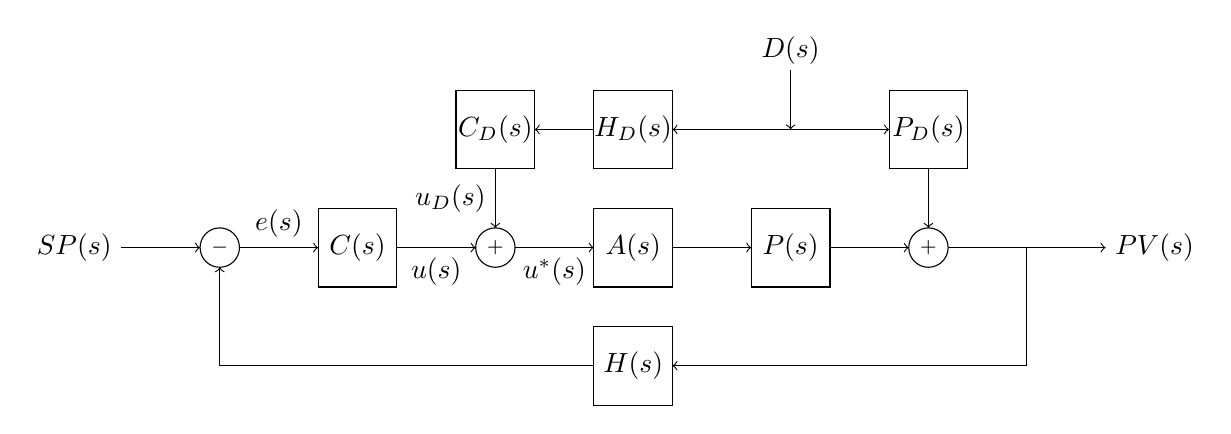
\begin{tikzpicture}
    
    %Error Sum
    \draw[->] (-4.5,0) node[anchor=east]{$SP(s)$}-- (-3.5,0);
    \draw (-3.25,0) circle (0.25) node{\scriptsize$-$};
    %Controller
    \draw[->] (-3,0) -- (-2,0)node[pos=0.5,anchor=south]{$e(s)$};
    \draw (-2,-0.5) rectangle (-1,0.5) node[pos=0.5]{$C(s)$};
    \draw[->] (-1,0) -- (0,0) node[pos=0.5,anchor=north]{$u(s)$};
    %Control Sum
    \draw (0.25,0) circle (0.25) node{\scriptsize$+$}; 
    %Actuator
    \draw[->] (0.5,0) -- (1.5,0)node[pos=0.5,anchor=north]{$u^*(s)$};
    \draw (1.5,-0.5) rectangle (2.5,0.5) node[pos=0.5]{$A(s)$};
    \draw[->] (2.5,0) -- (3.5,0);
    %Process
    \draw (3.5,-0.5) rectangle (4.5,0.5) node[pos=0.5]{$P(s)$};
    \draw[->] (4.5,0) -- (5.5,0);
    \draw[->] (6,0) -- (8,0)node[anchor=west]{$PV(s)$};
    %Output Sum
    \draw (5.75,0) circle (0.25) node{\scriptsize$+$};
    %Transducer
    \draw[->] (7,0) -- (7,-1.5) -- (2.5,-1.5);
    \draw (1.5,-2) rectangle (2.5,-1) node[pos=0.5]{$H(s)$} ;
    \draw[->] (1.5,-1.5) -- (-3.25,-1.5) -- (-3.25,-0.25);
    %Disturbance Transducer
    \draw (1.5,1) rectangle (2.5,2) node[pos=0.5]{$H_D(s)$} ;
    \draw[->] (1.5,1.5) -- (0.75,1.5);
    %Disturbance Controller
    \draw (-0.25,1) rectangle (0.75,2) node[pos=0.5]{$C_D(s)$};
    \draw[->] (0.25,1) -- (0.25,0.25)node[pos=0.5,anchor=east]{$u_D(s)$};
    %Disturbance Dynamics
    \draw (5.25,1) rectangle (6.25,2) node[pos=0.5]{$P_D(s)$};
    \draw[->] (5.75,1) -- (5.75,0.25);
    %Disturbance
    \node at (4,2.5) {$D(s)$};
    \draw[<->] (2.5,1.5) -- (5.25,1.5);
    \draw[->] (4,2.25) -- (4,1.5);
\end{tikzpicture}

    \caption[Feedback control loop with disturbance feedforward]{Feedback control loop with disturbance feedforward. It is identical to Fig. \ref{fig:tikz_feedback} with the addition of a disturbance ($D$) which effects the process variable ($PV$) according to the disturbance dynamics ($P_D$), and is measured by the disturbance transducer ($H_D$). The signal from $H_D$ is sent to the disturbance feedforward controller ($C_D$) who's output ($u_D$) is combined with ($u$) to form the total control output ($u^*$).}
    \label{fig:tikz_feedforward}
\end{figure}

In many processes, the process variable is effected by phenomena other than the actuator. These other phenomena are defined as disturbances. A well-tuned feedback controller is capable of disturbance rejection, but only after the disturbance causes error. In some cases, a disturbance feedforward controller may be added to the feedback controller to cause the actuator to counteract the effect of the disturbance before it occurs \cite[Ch. 10]{Bequette}. Fig. \ref{fig:tikz_feedforward} shows a feedback control loop with the addition of a disturbance feedforward controller.

The most prevalent disturbances that would effect the power output of the core of a \acs{msnb} are the temperature reactivity feedback effect common to all nuclear reactors and the flow reactivity specific to natural circulation driven  liquid fueled \acsp{msr} \cite{CarterNumerical}. 

Temperature reactivity feedback is dominated by Doppler Broadening, where the radiative capture resonance peaks of nuclides such as \U[238] are depressed to cover a wider epithermal neutron spectrum \cite[Ch. 2]{DH}. This results in a lower resonance escape probability \cite[Ch. 3]{DH} and a negative correlation between fuel temperature and fuel reactivity. Liquid fuels also have a high thermal-expansion coefficient, so higher core temperatures lead to lower heavy metal density and lower macroscopic fission cross-section in the core \cite{PetersonMS}.

Flow reactivity is driven by the advection of delayed neutron precursors \cite[Ch. 3]{Kerlin}. Not all fission neutrons are released promptly; sometimes an unstable nuclide which eventually decays by neutron emission produced instead. These unstable nuclides are called delayed neutron precursors and have half-lives ranging from less than a second to over a minute \cite[Ch. 7]{Lamarsh}. An example is given by \ref{rxn:delayed}

\begin{reaction}\label{rxn:delayed}
    {^{87}Br} \underset{56 sec}{\stackrel{\beta^-}{\longrightarrow}} {^{87}Kr^{*}} \to {^{86}Kr + n}
\end{reaction}

Since the fuel in a \acs{msnb} is flowing, some delayed neutron precursors will leave the core by advection before the neutron is emitted in a much less reactive part of the reactor. When the temperature differential between the core and primary heat exchanger is increased, the natural circulation flow rate increases too. This decreases the likelihood of delayed neutrons being emitted in the core, and negatively impacts core reactivity. Helix devices meant to elongate the in-core flow path may minimize delayed neutron losses \cite{CarterPHD}.

Disturbance feedforward will not be utilized in the design of the controller outlined in this work. When the outlet temperature of the heat exchanger is decreased, it takes time for the cooler salt to reach the core. The disturbance transport delay is on the order of minutes. Contrastly, Doppler Broadening has a nearly instantaneous effect, so disturbance dynamics are on the order of milliseconds, governed by the mean neutron lifetime \cite[Ch. 7]{Lamarsh}. The effect of control actuation are similarly prompt. Even with a temperature sensor just at the inlet of the core it would be nearly impossible to reliably predict the exact moment that control reactivity would be need to be inserted to counteract the temperature reactivity. 

\subsection{Pre-Filter}
\begin{figure}[!ht]
    \centering
    
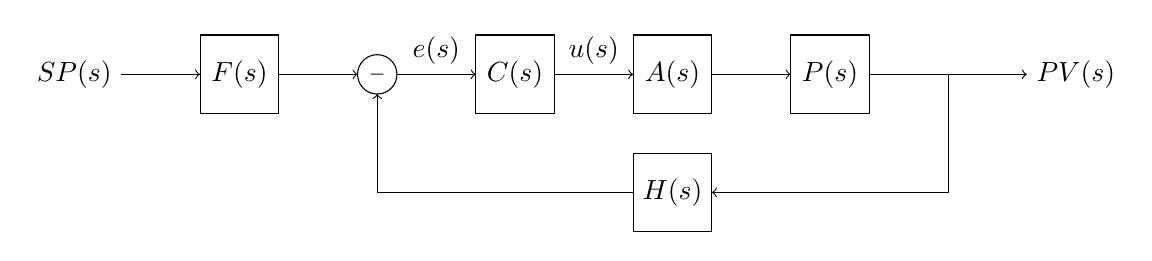
\begin{tikzpicture}
    %Pre-filter
    \draw[->] (-5,0)node[anchor=east]{$SP(s)$} -- (-4,0);
    \draw (-4,-0.5) rectangle (-3,0.5) node[pos=0.5]{$F(s)$};
    %Sum
    \draw[->] (-3,0) -- (-2,0);
    \draw (-1.75,0) circle (0.25) node{\scriptsize$-$};
    %Controller
    \draw[->] (-1.5,0) -- (-0.5,0)node[pos=0.5,anchor=south]{$e(s)$};
    \draw (-0.5,-0.5) rectangle (0.5,0.5) node[pos=0.5]{$C(s)$};
    \draw[->] (0.5,0) -- (1.5,0) node[pos=0.5,anchor=south]{$u(s)$};
    %Actuator
    \draw (1.5,-0.5) rectangle (2.5,0.5) node[pos=0.5]{$A(s)$};
    \draw[->] (2.5,0) -- (3.5,0);
    %Process
    \draw (3.5,-0.5) rectangle (4.5,0.5) node[pos=0.5]{$P(s)$};
    \draw[->] (4.5,0) -- (6.5,0) node[anchor=west]{$PV(s)$};
    %Transducer
    \draw[->] (5.5,0) -- (5.5,-1.5) -- (2.5,-1.5);
    \draw (1.5,-2) rectangle (2.5,-1) node[pos=0.5]{$H(s)$} ;
    \draw[->] (1.5,-1.5) -- (-1.75,-1.5) -- (-1.75,-0.25);
\end{tikzpicture}

    \caption[Feedback control loop with pre-filter]{Feedback control loop with pre-filter. It is identical to Fig. \ref{fig:tikz_feedback} with the addition of the pre-filter ($F$) which reshapes changes to the set-point ($SP$) before calculating the error ($e$).}
    \label{fig:tikz_prefilter}
\end{figure}

The control loop for a feedback system with a pre-filter is included as Fig. \ref{fig:tikz_prefilter}. Pre-filters are another type of feedforward mechanism common in control systems. They are typically first-order transfer functions such as \ref{eqn:prefilter} function used to improve the performance of the associated feedback controller (as depicted by Fig. \ref{fig:pgf_prefilter}) by `slowing down' the rate of change of the set-point. The gain (numerator) for a pre-filter is always unity because the desire is only to reshape the input, not resize it. The time-constant ($\tau_F$) describes how quickly the output equilibrates with the input. 

\begin{equation}\label{eqn:prefilter}
    F(s)=\frac{1}{\tau_F s+1}    
\end{equation}

\begin{figure}[!ht]
    \centering
    \subfloat[\centering Step-function]{{\resizebox{0.4\textwidth}{!}{% This file was created by matlab2tikz.
%
%The latest updates can be retrieved from
%  http://www.mathworks.com/matlabcentral/fileexchange/22022-matlab2tikz-matlab2tikz
%where you can also make suggestions and rate matlab2tikz.
%
\definecolor{mycolor1}{rgb}{0.00000,0.44700,0.74100}%
\definecolor{mycolor2}{rgb}{0.85000,0.32500,0.09800}%
%
\begin{tikzpicture}

\begin{axis}[%
width=4.521in,
height=3.566in,
at={(0.758in,0.481in)},
scale only axis,
xmin=0,
xmax=10,
xtick={ 0,  1,  2,  3,  4,  5,  6,  7,  8,  9, 10},
xticklabel style={font=\sansmath\sffamily},
xlabel style={font=\sansmath\sffamily},
xlabel={Time Constants, $\tau_F$},
ymin=-0.05,
ymax=1.05,
ylabel style={font=\sansmath\sffamily},
ylabel={Normalized Magnitude},
yticklabel style={font=\sansmath\sffamily},
ytick={0,0.632,0.865,0.95,1},
axis background/.style={fill=white},
legend style={at={(0.711,0.171)}, anchor=south west, legend cell align=left, align=left, font=\sansmath\sffamily}
]

\addplot [color=mycolor1]
  table[row sep=crcr]{%
0	0\\
0.2	0\\
0.4	0\\
0.6	0\\
0.8	0\\
0.999999999999993	0\\
1	1\\
1.00000000000001	1\\
1.20000000000001	1\\
1.40000000000001	1\\
1.60000000000001	1\\
1.80000000000001	1\\
2.00000000000001	1\\
2.20000000000001	1\\
2.40000000000001	1\\
2.60000000000001	1\\
2.80000000000001	1\\
3.00000000000002	1\\
3.20000000000002	1\\
3.40000000000002	1\\
3.60000000000002	1\\
3.80000000000002	1\\
4.00000000000002	1\\
4.20000000000002	1\\
4.40000000000002	1\\
4.60000000000002	1\\
4.80000000000002	1\\
4.99999999999996	1\\
5.00000000000002	1\\
5.20000000000002	1\\
5.40000000000002	1\\
5.60000000000002	1\\
5.80000000000002	1\\
6.00000000000002	1\\
6.20000000000002	1\\
6.40000000000002	1\\
6.60000000000002	1\\
6.80000000000002	1\\
7.00000000000002	1\\
7.20000000000002	1\\
7.40000000000002	1\\
7.60000000000002	1\\
7.80000000000002	1\\
8.00000000000002	1\\
8.20000000000002	1\\
8.40000000000002	1\\
8.60000000000002	1\\
8.80000000000002	1\\
9.00000000000002	1\\
9.20000000000002	1\\
9.40000000000001	1\\
9.60000000000001	1\\
9.80000000000001	1\\
10	1\\
};
\addlegendentry{Input}

\addplot [color=mycolor2, dashed]
  table[row sep=crcr]{%
0	0\\
0.2	0\\
0.4	0\\
0.6	0\\
0.8	0\\
0.999999999999993	0\\
1	0\\
1.00000000000001	1.42108547152019e-14\\
1.20000000000001	0.181269226666678\\
1.40000000000001	0.329679920797011\\
1.60000000000001	0.451188323173276\\
1.80000000000001	0.550670991417293\\
2.00000000000001	0.63212051332198\\
2.20000000000001	0.698805743378635\\
2.40000000000001	0.753402993352831\\
2.60000000000001	0.798103442046079\\
2.80000000000001	0.834701074973048\\
3.00000000000002	0.864664683281515\\
3.20000000000002	0.889196811483763\\
3.40000000000002	0.909282019778302\\
3.60000000000002	0.925726397897851\\
3.80000000000002	0.939189916312655\\
4.00000000000002	0.950212913156196\\
4.20000000000002	0.959237779886358\\
4.40000000000002	0.966626716003575\\
4.60000000000002	0.972676265384934\\
4.80000000000002	0.977629217628252\\
4.99999999999996	0.981684352048706\\
5.00000000000002	0.981684352048707\\
5.20000000000002	0.985004415388737\\
5.40000000000002	0.987722653414635\\
5.60000000000002	0.989948158535683\\
5.80000000000002	0.991770248064495\\
6.00000000000002	0.993262048833503\\
6.20000000000002	0.994483432030772\\
6.40000000000002	0.995483416040408\\
6.60000000000002	0.996302133721938\\
6.80000000000002	0.996972443082479\\
7.00000000000002	0.997521245983607\\
7.20000000000002	0.997970567807256\\
7.40000000000002	0.998338441411407\\
7.60000000000002	0.998639630851823\\
7.80000000000002	0.998886223915294\\
8.00000000000002	0.999088117244848\\
8.20000000000002	0.999253413526685\\
8.40000000000002	0.999388746679343\\
8.60000000000002	0.999499548096076\\
8.80000000000002	0.999590264625684\\
9.00000000000002	0.999664537040124\\
9.20000000000002	0.999725346151436\\
9.40000000000001	0.999775132442167\\
9.60000000000001	0.999815894010477\\
9.80000000000001	0.999849266760823\\
10	0.999876590058521\\
};
\addlegendentry{Output}

\end{axis}

\begin{axis}[%
width=5.833in,
height=4.375in,
at={(0in,0in)},
scale only axis,
xmin=0,
xmax=1,
ymin=0,
ymax=1,
axis line style={draw=none},
ticks=none,
axis x line*=bottom,
axis y line*=left
]
\end{axis}
\end{tikzpicture}%}}}
    \qquad
    \subfloat[\centering Ramp-function]{\resizebox{0.4\textwidth}{!}{% This file was created by matlab2tikz.
%
%The latest updates can be retrieved from
%  http://www.mathworks.com/matlabcentral/fileexchange/22022-matlab2tikz-matlab2tikz
%where you can also make suggestions and rate matlab2tikz.
%
\definecolor{mycolor1}{rgb}{0.00000,0.44700,0.74100}%
\definecolor{mycolor2}{rgb}{0.85000,0.32500,0.09800}%
%
\begin{tikzpicture}

  \begin{axis}[
    width=4.521in,
    height=3.566in,
    at={(0.758in,0.481in)},
    scale only axis,
    xmin=0,
    xmax=10,
    xtick={ 0,  1,  2,  3,  4,  5,  6,  7,  8,  9, 10},
    xticklabel style={font=\sansmath\sffamily},
    xlabel style={font=\sansmath\sffamily},
    xlabel={Time Constants, $\tau_F$},
    ymin=-0.05,
    ymax=1.05,
    ylabel style={font=\sansmath\sffamily},
    ylabel={Normalized Value},
    yticklabel style={font=\sansmath\sffamily},
    ytick={0,0.632,0.865,0.95,1},
    axis background/.style={fill=white},
    legend style={at={(0.711,0.171)}, anchor=south west, legend cell align=left, align=left, font=\sansmath\sffamily}
    ]
    
\addplot [color=mycolor1]
  table[row sep=crcr]{%
0	0\\
0.2	0\\
0.4	0\\
0.6	0\\
0.8	0\\
0.999999999999993	0\\
1	0\\
1.00000000000001	3.5527136788005e-15\\
1.20000000000001	0.0500000000000035\\
1.40000000000001	0.100000000000004\\
1.60000000000001	0.150000000000004\\
1.80000000000001	0.200000000000004\\
2.00000000000001	0.250000000000004\\
2.20000000000001	0.300000000000004\\
2.40000000000001	0.350000000000004\\
2.60000000000001	0.400000000000004\\
2.80000000000001	0.450000000000004\\
3.00000000000002	0.500000000000004\\
3.20000000000002	0.550000000000004\\
3.40000000000002	0.600000000000004\\
3.60000000000002	0.650000000000004\\
3.80000000000002	0.700000000000004\\
4.00000000000002	0.750000000000004\\
4.20000000000002	0.800000000000004\\
4.40000000000002	0.850000000000004\\
4.60000000000002	0.900000000000004\\
4.80000000000002	0.950000000000004\\
4.99999999999996	0.99999999999999\\
5.00000000000002	1\\
5.20000000000002	1\\
5.40000000000002	1\\
5.60000000000002	1\\
5.80000000000002	1\\
6.00000000000002	1\\
6.20000000000002	1\\
6.40000000000002	1\\
6.60000000000002	1\\
6.80000000000002	1\\
7.00000000000002	1\\
7.20000000000002	1\\
7.40000000000002	1\\
7.60000000000002	1\\
7.80000000000002	1\\
8.00000000000002	1\\
8.20000000000002	1\\
8.40000000000002	1\\
8.60000000000002	1\\
8.80000000000002	1\\
9.00000000000002	1\\
9.20000000000002	1\\
9.40000000000001	1\\
9.60000000000001	1\\
9.80000000000001	1\\
10	1\\
};
\addlegendentry{Input}

\addplot [color=mycolor2, dashed]
  table[row sep=crcr]{%
0	0\\
0.2	0\\
0.4	0\\
0.6	0\\
0.8	0\\
0.999999999999993	0\\
1	0\\
1.00000000000001	2.52378540224252e-29\\
1.20000000000001	0.00468269333333398\\
1.40000000000001	0.0175800198007507\\
1.60000000000001	0.0372029192066846\\
1.80000000000001	0.0623322521456803\\
2.00000000000001	0.0919698716695085\\
2.20000000000001	0.125298564155345\\
2.40000000000001	0.161649251661796\\
2.60000000000001	0.200474139488484\\
2.80000000000001	0.241324731256742\\
3.00000000000002	0.283833829179625\\
3.20000000000002	0.327700797129063\\
3.40000000000002	0.372679495055428\\
3.60000000000002	0.418568400525541\\
3.80000000000002	0.46520252092184\\
4.00000000000002	0.512446771710955\\
4.20000000000002	0.560190555028414\\
4.40000000000002	0.60834332099911\\
4.60000000000002	0.656830933653771\\
4.80000000000002	0.705592695592941\\
4.99999999999996	0.754578911987813\\
5.00000000000002	0.754578911987827\\
5.20000000000002	0.799066202819486\\
5.40000000000002	0.835489316845594\\
5.60000000000002	0.865310041159399\\
5.80000000000002	0.8897251858382\\
6.00000000000002	0.90971461612212\\
6.20000000000002	0.926080577836966\\
6.40000000000002	0.939479894328106\\
6.60000000000002	0.950450327081035\\
6.80000000000002	0.959432157972642\\
7.00000000000002	0.966785859324477\\
7.20000000000002	0.972806560919127\\
7.40000000000002	0.977735894591724\\
7.60000000000002	0.981771691761507\\
7.80000000000002	0.98507592309934\\
8.00000000000002	0.987781198977837\\
8.20000000000002	0.989996091589918\\
8.40000000000002	0.991809492331058\\
8.60000000000002	0.993294179322215\\
8.80000000000002	0.994509738250642\\
9.00000000000002	0.995504953752146\\
9.20000000000002	0.996319767309325\\
9.40000000000001	0.996986880243117\\
9.60000000000001	0.997533066131301\\
9.80000000000001	0.997980245325918\\
10	0.998346364693745\\
};
\addlegendentry{Output}

\end{axis}

\begin{axis}[%
width=5.833in,
height=4.375in,
at={(0in,0in)},
scale only axis,
xmin=0,
xmax=1,
ymin=0,
ymax=1,
axis line style={draw=none},
ticks=none,
axis x line*=bottom,
axis y line*=left
]
\end{axis}
\end{tikzpicture}%}}
    \caption[Pre-filter on (a) step-function and (b) ramp-function]{Pre-filter on step-function and ramp-function. When the pre-filter acts on a step-function, it follows an exponential curve, reaching 63.2\% of the magnitude of the step in 1 time constant, 86.5\% in 2 time constants, 95.0\% in 3 time constants and so on. The ramp-function exhibits similar but more complicated dynamics due to the changing input.}
    \label{fig:pgf_prefilter}
\end{figure}

By resisting instantaneous set-point changes, or step functions, the pre-filter minimizes the instantaneous error during transients and minimizes overshoot by reducing over-actuation or actuator saturation.  This is particularly useful in a control system such as the one designed in this report where the set-point is coupled to some other value. In this case, the core power generation needs to match the demand of the secondary system (\eg power cycle). This method allows the secondary system to immediately change to its necessary value while giving the reactor core time to safely and effectively respond. 

The area between the solid blue and dashed orange curves corresponds the net amount of energy expelled from the molten salt loop following the transient. This manifests as a drop in the average salt temperature. If the reactor begins to operate near thermophysical boundaries, it may be necessary for the core to over-produce in order to bring the temperature back up. An alternative approach could be to use a slightly under-damped second-order pre-filter so the core power generation briefly overshoots the heat exchanger power consumption to balance the energy inequality.

\section{Transport Delay Problem} 
A good place to start in the design of this controller is discussing the dynamics associated with anticipated transients. The prominent factors here are the natural circulation flow mode and the transport delay separating the heat exchanger and core. A common transient for the \acs{msnb} is a step-increase in power demand to a steady-state critical \acs{msnb} where the core power generation set-point is instantaneously equal to the heat exchanger power consumption. For this thought experiment, consider an ideal controller which produces rapid load following with minimal overshoot.

\begin{figure}[!ht]
    \centering
    \subfloat[\centering Immediate Response]{{\resizebox{0.30\textwidth}{!}{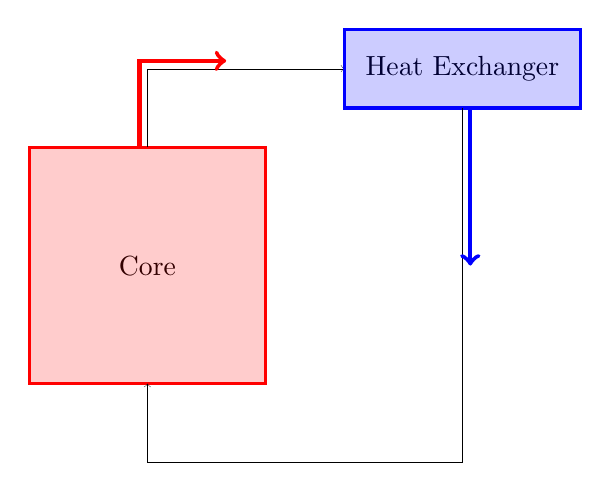
\begin{tikzpicture}
    %Core
    \draw node at (1.5,1.5) {Core};
    \draw[red, very thick] (0,0) rectangle (3,3);
    \filldraw[red,opacity=0.2] (0,0) rectangle (3,3) ;
    %Riser/Chimney
    \draw[->,ultra thin] (1.5,3) -- (1.5,4) -- (4,4); 
    \draw[->,ultra thick, red] (1.4,3) -- (1.4,4.1) -- (2.5,4.1);
    %HEX
    \draw node at (5.5,4) {Heat Exchanger};
    \draw[blue, very thick] (4,3.5) rectangle (7,4.5);
    \filldraw[blue,opacity=0.2] (4,3.5) rectangle (7,4.5) ;
    %Downcomer
    \draw[->, ultra thin] (5.5,3.5) -- (5.5,-1) -- (1.5,-1) -- (1.5,-1) -- (1.5,0);
    \draw[->,ultra thick, blue] (5.6,3.5) -- (5.6,1.5);
\end{tikzpicture}
}}}
    \qquad
    \subfloat[\centering Heat Exchanger Perturbation]{\resizebox{0.30\textwidth}{!}{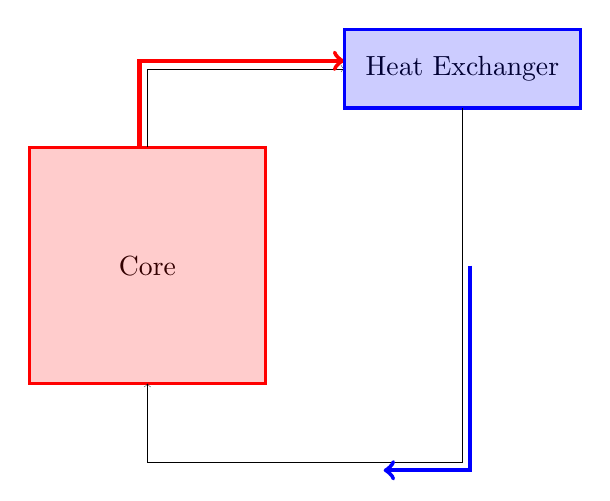
\begin{tikzpicture}
    %Core
    \draw node at (1.5,1.5) {Core};
    \draw[red, very thick] (0,0) rectangle (3,3);
    \filldraw[red,opacity=0.2] (0,0) rectangle (3,3) ;
    %Riser/Chimney
    \draw[->, ultra thin] (1.5,3) -- (1.5,4) -- (4,4); 
    \draw[->,ultra thick, red] (1.4,3) -- (1.4,4.1) -- (4,4.1);
    %HEX
    \draw node at (5.5,4) {Heat Exchanger};
    \draw[blue, very thick] (4,3.5) rectangle (7,4.5);
    \filldraw[blue,opacity=0.2] (4,3.5) rectangle (7,4.5) ;
    %Downcomer
    \draw[->, ultra thin] (5.5,3.5) -- (5.5,-1) -- (1.5,-1) -- (1.5,-1) -- (1.5,0);
    \draw[->,ultra thick, blue] (5.6,1.5) -- (5.6,-1.1) -- (4.5,-1.1);
\end{tikzpicture}
}}
    \subfloat[\centering Core Perturbations]{\resizebox{0.30\textwidth}{!}{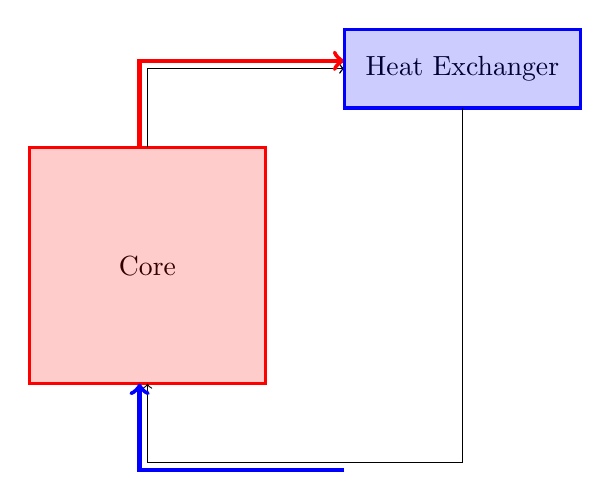
\begin{tikzpicture}
    %Core
    \draw node at (1.5,1.5) {Core};
    \draw[red, very thick] (0,0) rectangle (3,3);
    \filldraw[red,opacity=0.2] (0,0) rectangle (3,3) ;
    %Riser/Chimney
    \draw[->] (1.5,3) -- (1.5,4) -- (4,4); \draw[->] (1.5,3) -- (1.5,4) -- (4,4);
    \draw[->,ultra thick, red] (1.4,3) -- (1.4,4.1) -- (4,4.1);
    %HEX
    \draw node at (5.5,4) {Heat Exchanger};
    \draw[blue, very thick] (4,3.5) rectangle (7,4.5);
    \filldraw[blue,opacity=0.2] (4,3.5) rectangle (7,4.5) ;
    %Downcomer
    \draw[->] (5.5,3.5) -- (5.5,-1) -- (1.5,-1) -- (1.5,-1) -- (1.5,0);
    \draw[->,ultra thick, blue] (4,-1.1) -- (1.4,-1.1) -- (1.4,0);
\end{tikzpicture}
}}

    \caption[Transport Delay Problem Schematics]{Simplified schematic drawings of the transport delay problem in a natural circulation \acs{msnb}. These figures illustrate how an ideal controller would create hot (shown in red) and cold (shown in blue) `edges' in the temperature profile of the primary loop. These edges result in periodic disturbances in the form of sharp temperature reactivity insertions to the core, and are caused by three key events:
    \begin{enumerate*}[label=\alph*)]
        \item The instantaneous power changes upsetting the outlet temperature of both the core and heat exchanger;
        \item The first hot salt reaching the heat exchanger $\theta_{riser}$ after the power change; and
        \item The first cold salt reaching the core $\theta_{downcomer}$ after the power change;
    \end{enumerate*}
    It would take a very long time for these periodic disturbances to dampen with a controller that very quickly counteracts reactivity feedback.}
    \label{fig:thoughtexperiment}
\end{figure}

\subsection{Immediate Response}
The heat-exchanger immediately rejects more thermal energy to the secondary loop and the core immediately generates more power. The core outlet temperature increases quite sharply, but since there is a transport delay between the core outlet and heat exchanger inlet ($\theta_{riser}$), this hot salt does not instantaneously reach the heat exchanger, and the heat exchanger outlet temperature drops sharply. Thus, the heat exchanger outlet temperature also drops. 

As these hot and cold regions propagate and grow, the natural circulation driving force increases which results in a negative flow reactivity insertion. This is a gradual disturbance which the ideal controller can effectively reject by a counteracting insertion of positive control reactivity. 

\subsection{Heat Exchanger Perturbation}
Following the response to the initial step-increase, the first notable event occurs when the hot region in the riser reaches the heat exchanger. This produces a hot `edge' in the downcomer temperature profile that lags the cold edge by approximately $\theta_{riser}$, and again disturbs the core through a change in flow reactivity.

\subsection{Core Perturbations}
The next event occurs when the cold edge reaches the core inlet, $\theta_{downcomer}$ after the step-increase, causing a rapid insertion of positive temperature reactivity which must be rejected by the controller. $\theta_{riser}$ later, the hot edge inserts negative temperature reactivity. Each of these responses cause subsequent temperature edges which rise to the heat exchanger and continue through the system. It is apparent that the `ideal' controller actually inhibits the ability for the reactor to return to steady-state following a transient, instead prolonging both flow reactivity and temperature reactivity oscillations.

A pre-filter that reshapes the core set-point will make the initial hot edge more gradual. Proper tuning of the pre-filter time-constant will allow the reactivity oscillations to decay more quickly. Previous work \cite{CarterNumerical} has shown that the passive feedback mechanisms (temperature and flow reactivity) are capable of autonomous load following for small transient, though not at the level of performance that may be required in certain applications. Still, this provides the opportunity to minimize fine and rapid actuation while dampening oscillations by using a dead-band; the `ringing out' of minor perturbations could be left to the passive feedback mechanisms after the active feedback controls the bulk of the power change.

\section{Time-Variance and Non-Linearity}
In control systems, it is typically preferred to work with \acf{lti} systems. There are a number of non-linearities and time variances at play in the control of the \acs{msnb} which must be handled:

\begin{itemize}
    \item The Control Drum Angle vs. Reactivity Curve, which describes the relationship between control actuation and system response, is not linear, but sinusoidal \cite{PetersonMS}. Over small changes to the control drum angle, the curve may be linearized using Taylor Series approximation \cite[Ch. 2]{Bequette};
    \item The core reactivity decreases over the course of months and years due to the depletion of fissile nuclides \cite[Ch. 7]{Lamarsh}. This means that the bias-point (or unity-point) of the control drums will drift to provide less negative control reactivity. The bias-point, controller gain, and time constants will need to change with time. These parameters will be gain-scheduled according to the core's burn-up level, similarly to how autopilot systems for high-altitude aircraft account for the different air properties and mach-number at different altitudes \cite{GainSchedule};
    \item The control drums manipulate the criticality of the core, making it supercritical to increase the power, and subcritical to decrease. This is a highly time dependant exponential control mechanism. The derivative control time constant will need to be carefully tuned to minimize the likelihood of significant overshoot following a power transient; 
\end{itemize}


In addition to the relatively slow time variance of fissile fuel depletion during steady-state critical operation, there are specific times in a \acs{msnb}'s expected operational life-cycle that exhibit a higher degree of time variance: 
\begin{enumerate*}
\item Start-up; \item Shut-down; and \item Re-start.
\end{enumerate*}
\note{Samarium is Sm not Sa}
\subsection{Start-up}
Prior to start-up, it is very likely that the molten salt fuel/coolant mixture will need to be thawed. Initial start-up will also require a neutron source as a seed for the fission chain reaction \cite[Ch. 2]{DH}. Each of these systems are important considerations for the design of the \acs{msnb} and warrant further investigation, but are out of scope for this work and are briefly discussed in Chapter \ref{Chapter:Conclusions-FutureWork}. The key consideration regarding the start-up control system is the build-up of fission product neutron poisons in the first hours and days of operation.

\subsubsection{Xenon Poisoning}
\Xe is the strongest known neutron poison, with a microscopic neutron capture cross-section of 2.65 Mb \cite[Table II.2]{Lamarsh}. The concentration of \Xe is described by a system of differential equations which quantifies the generation, consumption, and decay of itself and its beta-precursor \I. Equations \ref{eqn:diffI} and \ref{eqn:diffXe} can be used to track the concentrations of iodine-135 and xenon-135 during start-up, steady-state operation, power transients, shut-down, and dead-time \cite[Ch. 7]{Lamarsh}.
\begin{equation}\label{eqn:diffI}
    \frac{dI}{dt} =
    \underbrace{\gamma_{I}\Sigma_{f}^{F}{\phi}(t)}_{\text{Fission Yield}}
    -\underbrace{\lambda_{I}I(t)}_{\text{Beta Decay}}
\end{equation}
\begin{equation}\label{eqn:diffXe}
        \frac{dXe}{dt} =
        \underbrace{\gamma_{Xe}\Sigma_{f}^{F}{\phi}(t)}_{\text{Fission Yield}}
        +
        \underbrace{\lambda_{I}I(t)}_{\text{Precursor Decay}}
        -
        \underbrace{\lambda_{Xe}Xe(t)}_{\text{Beta Decay}}
        -
        \underbrace{Xe(t)\sigma_{a}^{Xe}{\phi}(t)}_{\text{Radiative Capture}}
\end{equation}

Each nuclide is formed by \U[235] fission, and removed by beta-decay. Additionally, \Xe is formed by the beta-decay of \I and removed by radiative neutron capture\footnotemark. Each nuclide builds-up in the reactor until the formation terms, i.e. fission yield and precursor decay, equilibrate with the removal terms, beta decay and radiative capture. By setting the time derivatives to zero, the neutron flux dependent equilibrium concentrations (\ref{eqn:eqI} and \ref{eqn:eqXe}) may be derived algebraically \cite[Ch. 7]{Lamarsh} and can contribute over 2000 pcm of negative poison reactivity to the core. 

\footnotetext{In reality, the decay chain is a bit more complicated than this. $^{135}Te$, the direct beta-precursor to \I is formed by \U[235] fission \cite{Roberson}. It's half-life is orders of magnitude shorter than \I, so it is common to neglect its formation and instead lump its fission yield with \I. \Xe[135m] is also formed by \I beta-decay and is neglected for similar reasons.}
 
\begin{equation}\label{eqn:eqI}
    I_{\infty}(\phi) = \frac{\gamma_I \Sigma_f^F }{\lambda_I}\phi
\end{equation}
\begin{equation}\label{eqn:eqXe}
    Xe_{\infty}(\phi) = \frac{(\gamma_I+\gamma_{Xe}) \Sigma_f^F }{\lambda_I+\sigma_a^{Xe}\phi}\phi
\end{equation}

\subsubsection{Samarium Poisoning}
The second most important neutron poison to consider after \Xe is \Sa. \Pm is formed by fission\footnotemark and decays to \Sa, which is stable, and has a large neutron capture cross-section \cite[Ch. 7]{Lamarsh}. \ref{eqn:diffPm} looks identical to \ref{eqn:diffI}, but \ref{eqn:diffSa} is simpler than \ref{eqn:diffXe} as \Sa is stable and is not a direct fission product.

\footnotetext{As with \I, \Pm actually comes from the decay of a much shorter lived nuclide \Nd. Because neither \Pm nor \Nd are strong neutron absorbers, the presence of \Nd may be neglected in favor of its longer lived daughter product.}

\begin{equation}\label{eqn:diffPm}
    \frac{dPm}{dt} =
    \underbrace{\gamma_{Pm}\Sigma_{f}^{F}{\phi}(t)}_{\text{Fission Yield}}
    -\underbrace{\lambda_{Pm}Pm(t)}_{\text{Beta Decay}}
\end{equation}
\begin{equation}\label{eqn:diffSa}
        \frac{dSa}{dt} =
        \underbrace{\lambda_{Pm}Pm(t)}_{\text{Precursor Decay}}
        -
        \underbrace{Sa(t)\sigma_{a}^{Sa}{\phi}(t)}_{\text{Radiative Capture}}
\end{equation}

This system too reaches an equilibrium which may be found algebraically where the time derivatives are null. \ref{eqn:eqPm} is of the same form as \ref{eqn:eqI}. Interestingly \ref{eqn:eqSa} is independent of the neutron flux in the core. Because it is stable, it is only removed by the same neutron flux that forms it, and contributes a relatively constant 442 pcm of poison reactivity. 

\begin{equation}\label{eqn:eqPm}
    Pm_{\infty}(\phi) = \frac{\gamma_Pm \Sigma_f^F }{\lambda_{Pm}}\phi
\end{equation}
\begin{equation}\label{eqn:eqSa}
    Sa_{\infty}(\phi) = \frac{\gamma_{Pm} \Sigma_f^F }{\sigma_a^{Sa}}
\end{equation}

\subsubsection{Burnable Poison Control}
\acsp{lwr} are commonly controlled using neutron absorbing additives in two ways \cite[Ch. 8]{Kerlin}:
\begin{enumerate*}
    \item Burnable poisons (typically poisons who's daughter are neutron-transparent \cite[Ch. 14]{DH}) are placed in certain fuel rods to flatten the power profile; and 
    \item Soluble poisons (\ie chemical shim) dissolved in the moderator/coolant to account for non-equilibrium fission product poison build-up and fissile material depletion.
\end{enumerate*}

\acsp{msr} may be able to use the intersection of these two concepts; a neutron poison may be added to the molten salt mixture to counter-act the poison reactivity built-up by equilibrium poisons like \Xe and \Sa. Enough poison would need be added to the fuel salt to equate the reactivity of fresh fuel to the reactivity fuel with \Xe and \Sa at their equilibrium levels. There are many candidates for such a soluble poison, including boron-10 and isotopes of gadolinium, hafnium, and other lanthanides.

An ideal poison for this application should form a compound that is soluble in the molten salt at the desired level, and it should be burnt at a rate similar to the formation rate of its fission product counterpart. As the concentration of the fission product poisons build up, the concentration of the burnable poison depletes, and unlike chemical shimming, the consumed poison would not be replenished. Making the average core reactivity equivalent upon cold-clean start-up and equilibrium would simplify the gain and bias scheduling early in the fuel lifetime, particularly if the burnable poison has an appropriate effective half-life \cite{RootGd}.

\subsection{Shut-down}
Planned shut-down, either for scheduled maintenance or due to a lack of demand, is quite simple. The heat exchanger load is brought to zero or very low power, and the core set-point gradually follows. Careful tuning of the pre-filter time constant can alleviate potential thermal hydraulic (\eg stagnation or reverse-flow) and thermophysical (\eg salt precipitation, freezing, or vaporization) concerns \cite{CarterNumerical}. Whether the reactor is shut down for planned purposes or in an emergency, a decay heat \cite{TodreasKazimi1} removal system will need to be designed to keep the salt from vaporizing. The emergency shut-down (SCRAM) system and decay heat removal systems are briefly discussed in Chapter \ref{Chapter:Conclusions-FutureWork}.  

\subsection{Re-start}
Compound dynamics in the \Xe decay chain result in the generation of a large poison reactivity in the hours following a shut-down. This can make restarting the reactor difficult or impossible for a period of approximately two days. When the reactor is shut down, each flux-containing term in the system of ODEs (\ref{eqn:diffI} and \ref{eqn:diffXe}) goes to zero, and the concentrations of the two nuclides are described by the Bateman equations \cite{Bateman}, which have a readily available solution (\ref{eqn:I_inf} and \ref{eqn:Xe_inf}), given some initial condition \cite{Lamarsh}. \I follows simple exponential decay. \Xe has a longer half-life than \I, as well as a lower equilibrium concentration (owing to its huge radiative capture cross-section). This causes an inverse response, where the \Xe concentration initially spikes before its population grows and the \I population shrinks to the point that the rate of \Xe decay exceeds its formation. 

\begin{equation}\label{eqn:I_inf}
    I(t) = I_0e^{-\lambda_I t}
\end{equation}
\begin{equation}\label{eqn:Xe_inf}
    Xe(t) = Xe_0e^{-\lambda_{Xe} t}+\frac{\lambda_I I_0}{\lambda_I - \lambda_{Xe}}(e^{\lambda_{Xe}t}-e^{\lambda_{I}t})
\end{equation}

This system of equations is not ideal, as it results in mandatory reactor dead time. Most nuclear reactors are not designed with enough excess control reactivity to overcome the iodine pit, so they must wait for the xenon to decay. Even if the control system does have the ability to restart during the xenon peak, it can be very unsafe to do so. When the fission chain reaction is restarted, the neutron flux increases and begins transmuting \Xe. The removal of poisons is akin to positive reactivity insertion \cite{Roberson}. Decreasing poison concentration increases the neutron population and therefore the rate of poison removal. This is a positive feedback system which could run away quickly if control reactivity is not removed to match. 

The duration of the xenon spike may be shortened by adding an additional negative term to \ref{eqn:diffXe}. This is not physically realizable in cladded solid fuel reactors. It is however possible to remove a gaseous solvent from a liquid (such as \acs{msr} fuel) through a process called stripping \cite[Ch. 10]{Geankoplis}. Helium may be bubbled through the molten salt in a sparge tube, and the xenon (as well as any other fission gasses \cite{Offgas}) would preferentially transport into the gaseous phase which would later be separated in a cyclone or similar apparatus \cite{ORNL-masstransport}. This advective removal of \Xe would allow the \acs{msnb} to be restarted without having to wait for the poison to decay \cite{RootXe}. \Sa is stable and strongly dissolved in the molten salt, so it is always `burnt off' during restart \cite[Ch. 7]{Lamarsh}.